\section{Post-Training Objectives: From Preferences to Verifiable Rewards}

\begin{frame}{}
    \LARGE Alignment and Post-Training: \textbf{Objectives and Algorithms}

    \vspace{1em}
    \normalsize What replaced RLHF and DPO at the frontier, and why?
\end{frame}

\begin{frame}{Recap: The Starting Point}
    \begin{center}
    \small
    \begin{adjustbox}{max width=\linewidth}\begin{tabular}{l>{\raggedright\arraybackslash}p{4.0cm}c>{\raggedright\arraybackslash}p{5.6cm}}
        \toprule
        \textbf{Method} & \textbf{Data it needs} & \textbf{Models} & \textbf{Main risk} \\
        \midrule
        RLHF with PPO & pairs for a reward model, then rollouts & 4 & instability, reward over-optimisation \\
        DPO & preference pairs $(x, y_w, y_l)$ & 2 & offline, sensitive to the SFT start \\
        ORPO & preference pairs & 1 & no reference policy, so no KL leash \\
        KTO & unpaired thumbs up or down & 2 & weights must match the class balance \\
        \rowcolor{KAUSTcyan!12} GRPO & prompts and a reward function & no critic & today's topic \\
        \bottomrule
    \end{tabular}\end{adjustbox}
    \end{center}
    \[
        \mathcal{L}_{\text{DPO}}=-\,\mathbb{E}\Big[\log\sigma\Big(\beta\log\tfrac{\pi_\theta(y_w|x)}{\pi_{\text{ref}}(y_w|x)}-\beta\log\tfrac{\pi_\theta(y_l|x)}{\pi_{\text{ref}}(y_l|x)}\Big)\Big]
    \]
    \begin{itemize}\itemsep0.3em
        \item Today: what these methods \textbf{get wrong}, and what replaced them.
    \end{itemize}
    \src{Table after the KAUST Academy LLM course, ``Choosing a Preference Method''. DPO loss as written in Park et al., \href{https://arxiv.org/abs/2403.19159}{arXiv:2403.19159}. GRPO: Shao et al., ``DeepSeekMath,'' \href{https://arxiv.org/abs/2402.03300}{arXiv:2402.03300}.}
\end{frame}

\begin{frame}{One Map for Every Objective}
    \begin{itemize}\itemsep0.3em
        \item DeepSeekMath's \emph{unified paradigm}: every method has the same gradient, and differs in three choices.
    \end{itemize}
    \[
        \nabla_\theta\mathcal{J}_{\mathcal{A}}(\theta)=\mathbb{E}_{(q,o)\sim\textcolor{KAUSTblue}{\mathcal{D}}}\Big[\frac{1}{|o|}\sum_t \textcolor{KAred}{GC_{\mathcal{A}}}(q,o,t,\textcolor{darkorange}{\pi_{rf}})\,\nabla_\theta\log\pi_\theta(o_t|q,o_{<t})\Big]
    \]
    \begin{center}
    \small
    \begin{adjustbox}{max width=\linewidth}\begin{tabular}{llcc}
        \toprule
        \textbf{Method} & \textcolor{KAUSTblue}{\textbf{Data source}} & \textbf{On-policy} & \textbf{Negative gradient} \\
        \midrule
        SFT, offline best-of-$N$ & fixed dataset, $GC=1$ & \xmark & \xmark \\
        DPO, IPO and variants & fixed pairs & \xmark & \cmark \\
        ReST, online best-of-$N$ & live policy, filtered & \cmark & \xmark \\
        \rowcolor{KAUSTcyan!12} REINFORCE, PPO, GRPO & live policy, any reward & \cmark & \cmark \\
        \bottomrule
    \end{tabular}\end{adjustbox}
    \end{center}
    \begin{itemize}\itemsep0.3em
        \item Both axes do the same job: they make the update \textbf{mode-seeking}. If the reward peak lies where $\pi_{\text{ref}}$ puts little mass, you need on-policy samples to find it.
        \item DeepSeekMath's own finding: online data beats offline data, with everything else fixed.
    \end{itemize}
    \src{Shao et al., ``DeepSeekMath,'' \href{https://arxiv.org/abs/2402.03300}{arXiv:2402.03300}, Eq. 5 and Table 10. Tajwar et al., ``Preference Fine-Tuning of LLMs Should Leverage Suboptimal, On-Policy Data,'' ICML 2024, \href{https://arxiv.org/abs/2404.14367}{arXiv:2404.14367}, Table 1 (rows follow the paper's prose).}
\end{frame}

\begin{frame}{Offline Losses Are One Family: DPO, SLiC, IPO}
    \begin{columns}[T,onlytextwidth]
        \column{0.56\textwidth}
        \begin{itemize}\itemsep0.4em
            \item Let $\rho$ be the log-ratio gap between winner and loser. Each offline loss is $f(\beta\rho)$ for a convex $f$, a surrogate of the 0-1 loss.
            \item \textbf{Why IPO exists.} A preference observed once looks deterministic. Under Bradley-Terry that pushes $r(y_w)-r(y_l)\to\infty$, so $\pi(y_l)\to 0$ \emph{whatever} the regularisation strength.
            \item \textbf{IPO} regresses the gap onto a finite target instead:
            \[
                \mathcal{L}_{\text{IPO}}=\mathbb{E}\Big[\big(h_\pi(y_w,y_l,x)-\tfrac{1}{2\tau}\big)^2\Big]
            \]
        \end{itemize}
        \column{0.42\textwidth}
        \centering
        \begin{adjustbox}{max width=\linewidth}\begin{tikzpicture}
            \begin{axis}[width=6.4cm, height=4.6cm, xmin=-2, xmax=3, ymin=0, ymax=4,
                xlabel={\scriptsize $\beta\rho$}, ylabel={\scriptsize loss $f(\beta\rho)$},
                tick label style={font=\scriptsize}, axis lines=left,
                legend style={font=\scriptsize, draw=none, at={(0.5,1.02)}, anchor=south, legend columns=3}]
                \addplot[KAUSTblue, thick, domain=-2:3, samples=60] {ln(1+exp(-x))};
                \addplot[darkorange, thick, domain=-2:3, samples=60] {max(0,1-x)};
                \addplot[KAred, thick, domain=-1:3, samples=60] {(x-1)^2};
                \legend{DPO, SLiC, IPO}
            \end{axis}
        \end{tikzpicture}\end{adjustbox}
    \end{columns}
    \vspace{0.2em}
    \caveat{IPO's evidence is a 3-action bandit. The paper has \textbf{no LLM experiments}.}
    \src{Tang et al., ``Generalized Preference Optimization,'' \href{https://arxiv.org/abs/2402.05749}{arXiv:2402.05749}, Table 1. Azar et al., ``A General Theoretical Paradigm to Understand Learning from Human Preferences,'' \href{https://arxiv.org/abs/2310.12036}{arXiv:2310.12036}, Sec. 4.2 and Eq. 17.}
\end{frame}

\begin{frame}{SimPO: Train on What You Decode With}
    \begin{columns}[T,onlytextwidth]
        \column{0.6\textwidth}
        \begin{itemize}\itemsep0.4em
            \item \textbf{The mismatch.} DPO ranks by a log-ratio to $\pi_{\text{ref}}$. Decoding ranks by likelihood. Only about \alert{half} of DPO training triples agree on both.
            \item \textbf{SimPO} drops the reference model and uses the length-normalised log-likelihood as the reward, with a target margin $\gamma$:
        \end{itemize}
        \[
            \mathcal{L}=-\mathbb{E}\Big[\log\sigma\Big(\tfrac{\beta}{|y_w|}\log\pi_\theta(y_w|x)-\tfrac{\beta}{|y_l|}\log\pi_\theta(y_l|x)-\gamma\Big)\Big]
        \]
        \begin{itemize}\itemsep0.4em
            \item Length normalisation matters: the correlation between likelihood and length falls from 0.82 to 0.34.
            \item About 10\% less memory and 20\% less run time than DPO.
        \end{itemize}
        \column{0.38\textwidth}
        \centering
        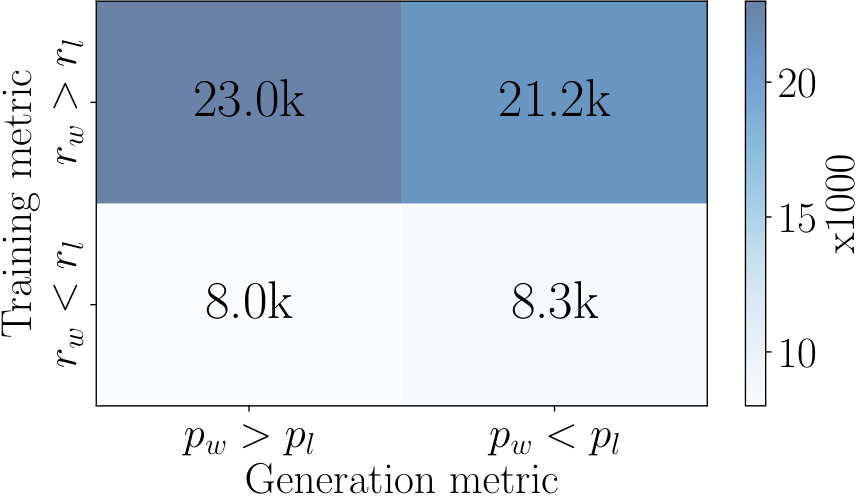
\includegraphics[width=\linewidth,height=0.42\textheight,keepaspectratio]{images/alignment-post-training/simpo_fig4_contingency_dpo.png}

        \vspace{0.2em}
        {\scriptsize DPO training pairs: reward ranking (rows) against likelihood ranking (columns).}
    \end{columns}
    \vspace{0.3em}
    \src{Meng, Xia, Chen, ``SimPO: Simple Preference Optimization with a Reference-Free Reward,'' \href{https://arxiv.org/abs/2405.14734}{arXiv:2405.14734}, Figures 4b and 5c, Table 6.}
\end{frame}

\begin{frame}{What Survived: Length-Normalised DPO}
    \begin{columns}[T,onlytextwidth]
        \column{0.4\textwidth}
        \centering
        \footnotesize
        \begin{adjustbox}{max width=\linewidth}\begin{tabular}{lr}
            \toprule
            \textbf{T\"ulu 3 ablation} & \textbf{Average} \\
            \midrule
            SFT checkpoint & 55.7 \\
            SimPO & 51.8, 52.9 \\
            DPO & 55.2 \\
            PPO & 54.5 to 55.5 \\
            \rowcolor{KAUSTcyan!12} DPO, length-norm. & 57.3 \\
            \bottomrule
        \end{tabular}\end{adjustbox}
        \column{0.58\textwidth}
        \begin{itemize}\itemsep0.35em
            \item SimPO's headline gains did not transfer. In T\"ulu 3, \emph{only} length-normalised DPO beat the SFT checkpoint.
            \item What the field kept is one idea from SimPO's appendix: \textbf{divide each log-ratio by its length}, and keep $\pi_{\text{ref}}$.
        \end{itemize}
    \end{columns}
    \vspace{0.3em}
    {\footnotesize Other variants, by the failure each one patches:}
    \begin{center}
    \footnotesize
    \begin{adjustbox}{max width=\linewidth}\begin{tabular}{llll}
        \toprule
        \textbf{Label noise} & \textbf{Likelihood displacement} & \textbf{Static $\beta$} & \textbf{Distribution shift} \\
        \midrule
        cDPO, Robust DPO & DPOP, RPO, CPO & $\beta$-DPO & iterative and online DPO \\
        \bottomrule
    \end{tabular}\end{adjustbox}
    \end{center}
    \takeaway{Lambert's verdict: ``the choice of algorithm is far less important than the initial model and the data used''.}
    \src{Lambert et al., ``T\"ulu 3,'' \href{https://arxiv.org/abs/2411.15124}{arXiv:2411.15124}, Table 18. SimPO repository. Hugging Face TRL paper index. Lambert, RLHF Book, ``Direct-Alignment Algorithms''.}
\end{frame}

\begin{frame}{Offline or Online? The Quantified Evidence}
    \begin{center}
    \small
    \begin{adjustbox}{max width=\linewidth}\begin{tabular}{lcccc}
        \toprule
        \textbf{Benchmark} & \textbf{SFT} & \textbf{DPO} & \textbf{Iterative DPO} & \textbf{PPO} \\
        \midrule
        CodeContests, 10@1k (\%) & 15.2 & \alert{0.0} & 3.2 & \textbf{22.4} \\
        APPS introductory, pass@5 (\%) & 38.6 & n/a & 34.2 & \textbf{44.4} \\
        SafeRLHF helpfulness reward & n/a & $-2.86$ & $-2.96$ & $\mathbf{+1.69}$ \\
        SafeRLHF safety rate (\%) & n/a & 95.8 & 99.9 & 99.5 \\
        \bottomrule
    \end{tabular}\end{adjustbox}
    \end{center}
    \begin{itemize}\itemsep0.4em
        \item \textbf{Theory.} The policies PPO can reach are a proper subset of those DPO can reach. DPO is free to exploit out-of-distribution responses.
        \item \textbf{The counterpoint is cost.} In T\"ulu 3, PPO took about 28 hours on two nodes against 4 hours on one for DPO, for similar scores.
    \end{itemize}
    \takeaway{A spectrum, not a binary: offline DPO, iterative DPO, online DPO, PPO and GRPO. On-policy pays most when the reward is \textbf{accurate} and the task is \textbf{hard}.}
    \src{Xu et al., ``Is DPO Superior to PPO for LLM Alignment?'' ICML 2024, \href{https://arxiv.org/abs/2404.10719}{arXiv:2404.10719}, Tables 6 to 8. Guo et al., ``Direct Language Model Alignment from Online AI Feedback,'' \href{https://arxiv.org/abs/2402.04792}{arXiv:2402.04792}. T\"ulu 3, \href{https://arxiv.org/abs/2411.15124}{arXiv:2411.15124}.}
\end{frame}

\begin{frame}{From PPO to GRPO: Delete the Critic}
    \begin{itemize}\itemsep0.35em
        \item PPO for LLMs keeps \textbf{four or five models} in memory: policy, old policy, reference, value and reward model.
        \item GAE needs one value call per token. With 512 prompts, 16 responses and about 2,000 tokens each, that is roughly \alert{16 million value forward passes per step}.
        \item \textbf{GRPO} replaces the critic with the statistics of a group of $G$ samples for the same prompt:
    \end{itemize}
    {\footnotesize\[
        \mathcal{J}=\mathbb{E}\Big[\frac{1}{G}\sum_{i}\frac{1}{|o_i|}\sum_t\min\big(r_{i,t}\hat A_{i,t},\,\mathrm{clip}(r_{i,t},1-\varepsilon,1+\varepsilon)\hat A_{i,t}\big)\Big]-\beta D_{KL},
        \qquad
        \hat A_{i,t}=\frac{R_i-\mathrm{mean}(\{R_j\})}{\mathrm{std}(\{R_j\})}
    \]}
    \begin{itemize}\itemsep0.35em
        \item $r_{i,t}$ is the token probability ratio to the policy that sampled. Every token of a response gets the same advantage.
        \item Three terms have since been \textbf{questioned}: $1/|o_i|$, the division by std, and the KL term.
    \end{itemize}
    \src{Choi, Stanford CS224N Lecture 12 (2026). Hashimoto, Stanford CS336 Lecture 16 (2025). Objective as written in ``DAPO,'' \href{https://arxiv.org/abs/2503.14476}{arXiv:2503.14476}, Eqs. 8 to 9, after Shao et al., \href{https://arxiv.org/abs/2402.03300}{arXiv:2402.03300}.}
\end{frame}

\begin{frame}{GRPO's Hidden Biases (Dr. GRPO)}
    \begin{columns}[T,onlytextwidth]
        \column{0.5\textwidth}
        \textbf{Length bias, from $1/|o_i|$}
        \begin{itemize}\itemsep0.35em
            \item Short correct answers get larger updates.
            \item Long \emph{wrong} answers are penalised less. So wrong answers grow longer during training.
            \item Not specific to GRPO: the PPO losses in TRL, OpenRLHF and verl all normalised by length.
        \end{itemize}
        \column{0.47\textwidth}
        \textbf{Difficulty bias, from dividing by std}
        \begin{itemize}\itemsep0.35em
            \item Prompts that are almost always solved, or almost never, have a small std.
            \item Their advantages are inflated, so the easiest and hardest questions dominate.
            \item The std is ``not a valid baseline''. It breaks unbiasedness.
        \end{itemize}
    \end{columns}
    \vspace{0.5em}
    \[
        \textbf{Fix:}\qquad \tilde A_i = R_i-\mathrm{mean}(\{R_j\}), \qquad \text{sum over tokens, divide by a constant}
    \]
    \begin{itemize}\itemsep0.35em
        \item Result: a 7B model reaches 43.3\% on AIME 2024 in 27 hours on 8 A100 GPUs.
        \item A side finding that deflates a famous story: the base model already shows the ``aha moment'' before any RL.
    \end{itemize}
    \src{Liu et al., ``Understanding R1-Zero-Like Training: A Critical Perspective,'' COLM 2025, \href{https://arxiv.org/abs/2503.20783}{arXiv:2503.20783}, Sec. 3.1 and Table 2. Hashimoto, Stanford CS336 Lecture 16 (2025).}
\end{frame}

\begin{frame}{DAPO: Four Fixes, Twenty Points}
    \begin{columns}[T,onlytextwidth]
        \column{0.5\textwidth}
        \centering
        \begin{adjustbox}{max width=\linewidth}\begin{tikzpicture}
            \begin{axis}[ybar, width=7.4cm, height=5.6cm, bar width=0.5cm,
                ymin=20, ymax=56, ylabel={\scriptsize AIME 2024, avg@32},
                symbolic x coords={A,B,C,D,E,F}, xtick=data,
                xticklabels={naive GRPO, + overlong filter, + clip-higher, + soft length penalty, + token-level loss, + dynamic sampling},
                x tick label style={font=\tiny, rotate=25, anchor=east},
                y tick label style={font=\scriptsize},
                nodes near coords, nodes near coords style={font=\scriptsize},
                axis lines=left, enlarge x limits=0.12]
                \addplot[fill=KAUSTcyan!55, draw=KAUSTcyan!70!black] coordinates {(A,30) (B,36) (C,38) (D,41) (E,42) (F,50)};
            \end{axis}
        \end{tikzpicture}\end{adjustbox}
        \column{0.48\textwidth}
        \begin{itemize}\itemsep0.45em
            \item \textbf{Clip-higher.} Asymmetric clip, $\varepsilon_{low}=0.2$ and $\varepsilon_{high}=0.28$, to counter early entropy collapse.
            \item \textbf{Dynamic sampling.} Drop prompts whose group is all correct or all wrong. They carry no gradient.
            \item \textbf{Token-level loss.} Average over all tokens of the batch, not per sample.
            \item \textbf{Overlong shaping.} Mask or softly punish truncated responses.
            \item \textbf{No KL term.} A long-reasoning model must move far from its start.
        \end{itemize}
    \end{columns}
    \vspace{0.2em}
    \src{ByteDance Seed and Tsinghua AIR, ``DAPO: An Open-Source LLM Reinforcement Learning System at Scale,'' \href{https://arxiv.org/abs/2503.14476}{arXiv:2503.14476}, Table 1 (Qwen2.5-32B base). The final 50 beats DeepSeek-R1-Zero-Qwen-32B (47) with half the steps.}
\end{frame}

\begin{frame}{Does RL Just Trade Entropy for Performance?}
    \centering
    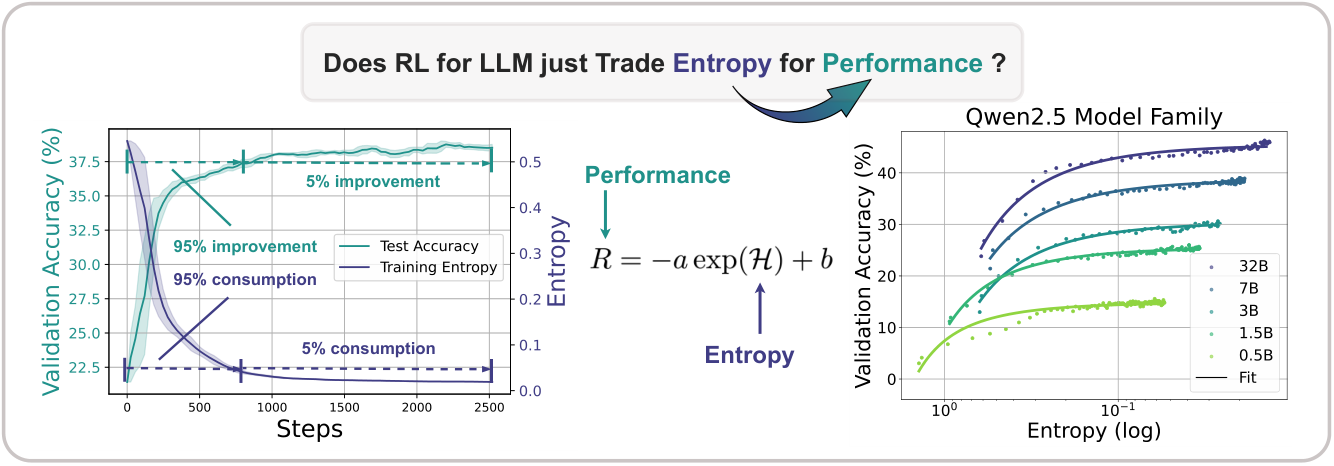
\includegraphics[width=0.78\linewidth,height=0.36\textheight,keepaspectratio]{images/alignment-post-training/entropy_fig1_collapse.png}
    \begin{itemize}\itemsep0.3em
        \item An empirical law across 11 models: $R=-a\,e^{H}+b$. Reward rises only as policy entropy $H$ falls, so the ceiling is fixed at $H=0$.
        \item 73\% of the entropy drop and 76\% of the gain happen in the \alert{first 200 steps}, one twelfth of training.
        \item \textbf{Fixes that keep exploration alive.} Clip-Cov and KL-Cov restrain only high-covariance tokens. CISPO clips the importance weight, not the update, so rare ``fork'' tokens such as \emph{However} keep their gradient.
    \end{itemize}
    \src{Cui et al., ``The Entropy Mechanism of Reinforcement Learning for Reasoning Language Models,'' \href{https://arxiv.org/abs/2505.22617}{arXiv:2505.22617}, Figures 1 and 2. MiniMax, ``MiniMax-M1,'' \href{https://arxiv.org/abs/2506.13585}{arXiv:2506.13585}.}
\end{frame}

\begin{frame}{The Policy-Gradient Family on One Table}
    \begin{center}
    \small
    \begin{adjustbox}{max width=\linewidth}\begin{tabular}{llll}
        \toprule
        \textbf{Method} & \textbf{Importance sampling} & \textbf{Clipping} & \textbf{Advantage or baseline} \\
        \midrule
        REINFORCE & none & none & Monte Carlo baseline \\
        RLOO & none & none & leave-one-out \\
        PPO & token level & two-sided & learned value function \\
        GRPO & token level & two-sided & group-relative \\
        GSPO & sequence level & two-sided & group-relative \\
        \rowcolor{KAUSTcyan!12} CISPO & token level & stop-gradient on the weight & group-relative \\
        \bottomrule
    \end{tabular}\end{adjustbox}
    \end{center}
    \begin{itemize}\itemsep0.25em
        \item \textbf{Two rollouts can be enough.} GRPO with $G=2$ is a contrastive, DPO-like objective. It keeps 97.6\% of the performance of $G=16$ with 12.5\% of the rollouts.
        \item \textbf{Normalise over the batch, not the prompt.} With per-prompt normalisation, one GRPO run scored 95.0 on its AIME-24 training set and \alert{0.0} on AIME-25.
        \item \textbf{The critic is not dead.} VAPO repairs value-based PPO with value pre-training and a length-adaptive GAE: 5 to 60 on AIME 2024.
    \end{itemize}
    \src{Table: Lambert, RLHF Book, ``Reinforcement Learning''. Wu et al., ``It Takes Two: Your GRPO Is Secretly DPO,'' \href{https://arxiv.org/abs/2510.00977}{arXiv:2510.00977}. Hu et al., ``REINFORCE++,'' \href{https://arxiv.org/abs/2501.03262}{arXiv:2501.03262}. ByteDance Seed, ``VAPO,'' \href{https://arxiv.org/abs/2504.05118}{arXiv:2504.05118}.}
\end{frame}

\begin{frame}{The Sampler Is Not the Learner}
    \begin{itemize}\itemsep0.4em
        \item Rollouts come from an inference engine. Gradients come from a training framework. Their token probabilities \textbf{differ even when the weights are identical}.
    \end{itemize}
    \begin{center}
    \small
    \begin{adjustbox}{max width=\linewidth}\begin{tabular}{>{\raggedright\arraybackslash}p{4.0cm}>{\raggedright\arraybackslash}p{9.3cm}}
        \toprule
        \textbf{Source of mismatch} & \textbf{Fix reported} \\
        \midrule
        Numerical precision of logits & compute the LM head in FP32: asymptotic reward 0.52 to 0.61 (ScaleRL) \\
        Engine and trainer log-probs & truncated importance sampling on the ratio between them (Olmo 3) \\
        MoE routing differs & \emph{Keep Routing}: replay the inference-time routes in training (DeepSeek-V3.2) \\
        Top-$p$ and top-$k$ truncation & \emph{Keep Sampling Mask}: apply the same mask in training (DeepSeek-V3.2) \\
        \bottomrule
    \end{tabular}\end{adjustbox}
    \end{center}
    \begin{itemize}\itemsep0.4em
        \item ScaleRL, after 400,000 GPU-hours of ablations: most tricks change \emph{efficiency}. Few move the \emph{asymptote}.
    \end{itemize}
    \src{Khatri et al., ``The Art of Scaling Reinforcement Learning Compute for LLMs,'' \href{https://arxiv.org/abs/2510.13786}{arXiv:2510.13786}. DeepSeek-AI, ``DeepSeek-V3.2,'' \href{https://arxiv.org/abs/2512.02556}{arXiv:2512.02556}. Olmo Team, ``Olmo 3,'' \href{https://arxiv.org/abs/2512.13961}{arXiv:2512.13961}.}
\end{frame}

\begin{frame}{What Labs Report Shipping}
    \begin{center}
    \footnotesize
    \renewcommand{\arraystretch}{1.2}
    \begin{adjustbox}{max width=\linewidth}\begin{tabular}{l>{\raggedright\arraybackslash}p{10.6cm}}
        \toprule
        \textbf{Model} & \textbf{Reported post-training recipe} \\
        \midrule
        T\"ulu 3 (Nov 2024) & SFT, length-normalised DPO on 354,192 on-policy pairs, then RLVR with PPO \\
        Llama 4 (Apr 2025) & light SFT, online RL on medium and hard prompts, light DPO for corner cases \\
        Qwen3 (May 2025) & GRPO on 3,995 query-verifier pairs. Small models by on-policy distillation \\
        Kimi K2 (Jul 2025) & a squared-loss policy objective, with a self-critique rubric reward \\
        GLM-4.5 (Aug 2025) & GRPO ``excluding the KL loss term'', with a two-stage difficulty curriculum \\
        DeepSeek-V3.2 (Dec 2025) & GRPO with unbiased KL, off-policy masking, Keep Routing and Keep Sampling Mask \\
        \rowcolor{KAUSTcyan!12} Olmo 3 (Dec 2025) & SFT, DPO with delta learning, then GRPO with no KL, no std, token-level loss, clip-higher \\
        \bottomrule
    \end{tabular}\end{adjustbox}
    \end{center}
    \begin{itemize}\itemsep0.35em
        \item \textbf{The trend:} the KL-to-reference anchor that defined RLHF and DPO is largely gone from RL recipes with verifiable rewards.
        \item \textbf{DPO changed jobs.} It went from \emph{the} alignment algorithm to a cheap stage before or after RL.
    \end{itemize}
    \src{Technical reports of each model: \href{https://arxiv.org/abs/2411.15124}{arXiv:2411.15124}, \href{https://arxiv.org/abs/2505.09388}{2505.09388}, \href{https://arxiv.org/abs/2507.20534}{2507.20534}, \href{https://arxiv.org/abs/2508.06471}{2508.06471}, \href{https://arxiv.org/abs/2512.02556}{2512.02556}, \href{https://arxiv.org/abs/2512.13961}{2512.13961}. Meta AI, ``The Llama 4 herd'' (2025). Lambert, RLHF Book.}
\end{frame}

\begin{frame}{Cheaper Than RL: On-Policy Distillation}
    \begin{columns}[T,onlytextwidth]
        \column{0.55\textwidth}
        \begin{itemize}\itemsep0.45em
            \item If a strong teacher exists, do you need a reward at all?
            \item \textbf{On-policy distillation.} The \emph{student} samples. The teacher scores every token. Minimise the per-token reverse KL on the states the student visits:
            \[
                \mathrm{KL}\big(\pi_\theta\,\|\,\pi_{\text{teacher}}\big)
            \]
            \item \textbf{Why on-policy.} Offline imitation compounds error as $O(\epsilon L^2)$ over a length-$L$ output. On-policy correction keeps it at $O(\epsilon L)$.
            \item Distillation also raised pass@64. RL did not.
            \item 2026: multi-teacher distillation (MOPD) beats mixed RL, cascaded RL and weight merging.
        \end{itemize}
        \column{0.42\textwidth}
        \centering
        \small
        \begin{adjustbox}{max width=\linewidth}\begin{tabular}{lcc}
            \toprule
            \textbf{Qwen3-8B} & \textbf{AIME'24} & \textbf{GPU-h} \\
            \midrule
            RL & 67.6 & 17,920 \\
            \rowcolor{KAUSTcyan!12} On-policy distillation & 74.4 & 1,800 \\
            \bottomrule
        \end{tabular}\end{adjustbox}

        \vspace{0.8em}
        {\scriptsize About one tenth of the compute, and a higher score.}
    \end{columns}
    \vspace{0.3em}
    \src{Qwen Team, ``Qwen3 Technical Report,'' \href{https://arxiv.org/abs/2505.09388}{arXiv:2505.09388}, Table 21. Lu, ``On-Policy Distillation'' (Thinking Machines, 2025). Lambert, RLHF Book, ``Synthetic Data and Distillation''. Ma et al., ``MOPD,'' \href{https://arxiv.org/abs/2606.30406}{arXiv:2606.30406}.}
\end{frame}

\begin{frame}{Objectives: What to Remember}
    \begin{center}
    \small
    \begin{adjustbox}{max width=\linewidth}\begin{tabular}{ll}
        \toprule
        \textbf{Symptom in an RL run} & \textbf{Fix} \\
        \midrule
        Wrong answers grow longer & drop $1/|o|$: Dr. GRPO, token-level loss \\
        Entropy collapses early & clip-higher, CISPO, Clip-Cov and KL-Cov \\
        Groups all correct or all wrong & dynamic or active sampling \\
        Divergence with a fast engine or MoE & importance correction, FP32 head, Keep Routing \\
        \bottomrule
    \end{tabular}\end{adjustbox}
    \end{center}
    \begin{itemize}\itemsep0.45em
        \item Offline preference losses are one family. \textbf{Length-normalised DPO} is the variant that lasted.
        \item The 2026 consensus for RL: GRPO \textbf{minus KL, minus std}, plus token-level loss, clip-higher and sample filtering.
    \end{itemize}
    \vspace{0.2em}
    \takeaway{\textbf{Next.} Every method here assumed a reward $R$ worth maximising. Where does $R$ come from, and what happens when the model finds its flaws?}
    \src{Diagnostic map compiled from the sources of this section. Wolfe, ``GRPO++: Tricks for Making RL Actually Work'' (2026).}
\end{frame}
